To give credibility to the approach mentioned in Chapter 3, a simple test case to test the capabilities of HTM and confirm that they apply on a video is introduced.
\section{Bouncing Ball Test}

\begin{figure}[H]
    \centering
    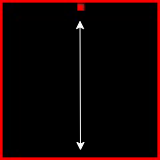
\includegraphics[width=.3\textwidth]{resources/experiments/bouncing_ball/bb_updown1.png}\hfill
    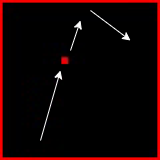
\includegraphics[width=.3\textwidth]{resources/experiments/bouncing_ball/bb_updownside.png}\hfill
    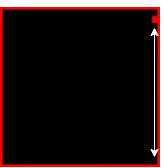
\includegraphics[width=.3\textwidth]{resources/experiments/bouncing_ball/bb_updown2.png}
    \caption{The bouncing ball test, and its three stages}
    \label{fig:bb}
\end{figure}
The video consists of a ball bouncing up and down until an anomaly occurs in the form of a sudden introduction of a horizontal velocity. After a while this horizontal velocity goes back to 0 and the ball goes back to bouncing up and down in-place.
\begin{figure}[H]
    \centering
    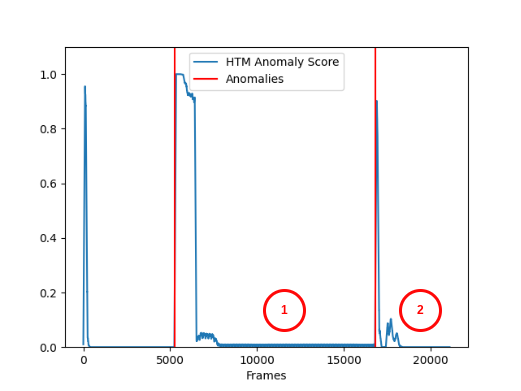
\includegraphics[width=\textwidth]{resources/experiments/bouncing_ball/bb_anoms_bad.png}
    \caption{The moving average of the anomaly score in the bouncing ball experiment.}
\end{figure}
From the figure, it can be observed that it correctly detects anomalies and quickly adapts to them. On the other hand, the result is not perfect due to the minor oscillations around frame 10000 and the anomaly spikes towards the end. \par
The reason for the oscillations is due to the spatial pooler being dominated by a lucky few columns. The solution is to enable boosting.\par
\begin{figure}[H]
    \centering
    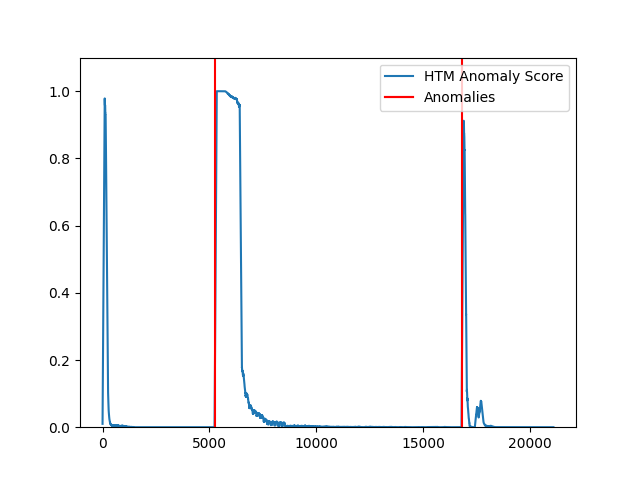
\includegraphics[width=\textwidth]{resources/experiments/bouncing_ball/bb_anoms_boosting.png}
    \caption{Bouncing ball with boosting enabled.}
\end{figure}
The reason for the anomaly spikes towards the end is because the spatial pooler had found an optimal representation when the ball was bouncing freely, but when the ball stops and starts bouncing in-place the spatial pooler ends up unlearning the old representation while it learns the new representation. This causes a sudden minor change in the SP output, which the TM reports as anomalous. The solution is to set the value by which permanence is decreased by to zero, effectively disabling the ability of the spatial pooler to "forget". This ability is important in HTM systems, so disabling it is not always feasible.
\begin{figure}[H]
    \centering
    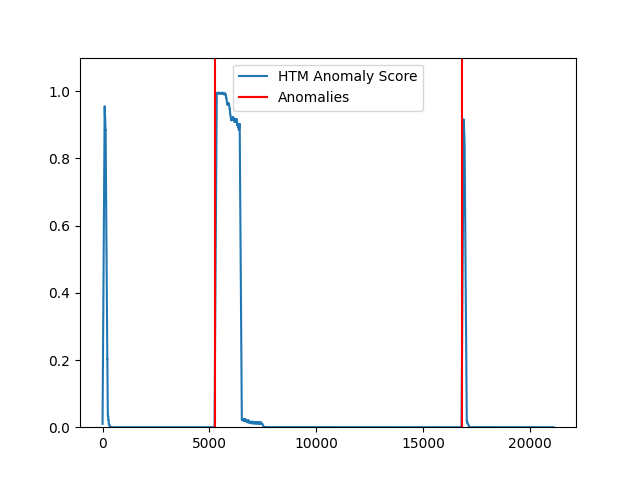
\includegraphics[width=\textwidth]{resources/experiments/bouncing_ball/bb_anoms_unforgetting.png}
    \caption{Bouncing ball without the ability of the SP to "forget".}
\end{figure}
\begin{figure}[H]
    \centering
    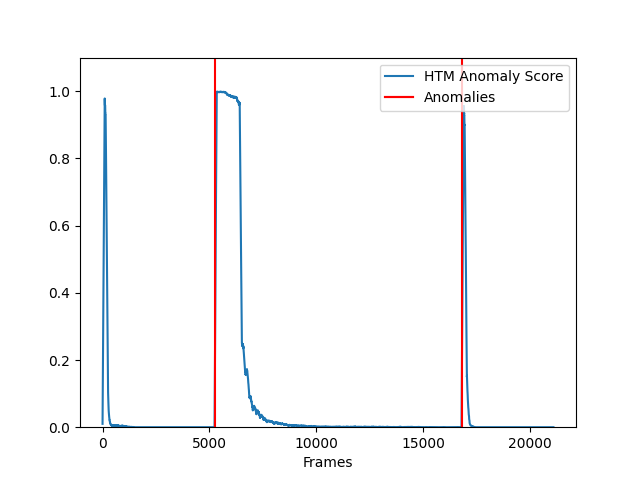
\includegraphics[width=\textwidth]{resources/experiments/bouncing_ball/bb_anoms_unforgetting_boosting.png}
    \caption{Bouncing ball without the ability of the SP to "forget" and with boosting enabled.}
\end{figure}
\section{Surveillance example}